\documentclass{sigplanconf}
%\documentclass{sig-alternate}
\usepackage{epsfig, times, graphicx, amssymb, amsmath, amsfonts}

\newcommand{\mt}[1]{\mbox{\it #1}}

\begin{document}

\conferenceinfo{LCTES'05,} {June 15--17, 2005, Chicago, Illinois, USA.}
\CopyrightYear{2005}
\copyrightdata{1-59593-018-3/05/0006} 

\title{Cache Aware Optimization of Stream Programs}
\authorinfo{Janis Sermulins \and William Thies \and Rodric Rabbah \and Saman Amarasinghe}
	     {Computer Science and Artificial Intelligence Laboratory, Massachusetts Institute of Technology}
	     {\{janiss, thies, rabbah, saman\}@csail.mit.edu}

\maketitle

\begin{abstract}
Effective use of the memory hierarchy is critical for achieving high
performance on embedded systems.  We focus on the class of streaming
applications, which is increasingly prevalent in the embedded domain.  We
exploit the widespread parallelism and regular communication patterns
in stream programs to formulate a set of cache aware optimizations
that automatically improve instruction and data locality.  Our work is
in the context of the Synchronous Dataflow model, in which a program
is described as a graph of independent actors that communicate over
channels.  The communication rates between actors are known at compile
time, allowing the compiler to statically model the caching behavior.

We present three cache aware optimizations: 1) execution scaling,
which judiciously repeats actor executions to improve instruction
locality, 2) cache aware fusion, which combines adjacent actors while
respecting instruction cache constraints, and 3) scalar replacement,
which converts certain data buffers into a sequence of scalar
variables that can be register allocated.  The optimizations are
founded upon a simple and intuitive model that quantifies the temporal
locality for a sequence of actor executions.  Our implementation of
cache aware optimizations in the StreamIt compiler yields a 249\%
average speedup (over unoptimized code) for our streaming benchmark
suite on a StrongARM 1110 processor.  The optimizations also yield a
154\% speedup on a Pentium~3 and a 152\% speedup on an Itanium~2.

\end{abstract}

\category{D.3.4}{Programming Languages}{Processors}[Optimization; code generation; compilers]
\category{D.3.2}{Programming Languages}{Language Classifications}[Concurrent, distributed, and parallel languages; Data-flow languages]
%\category{D.2.2}{Software Engineering}{Software Architectures, Design Tools and Techniques}

\terms 
Languages, Design, Performance

\keywords
Stream Programing, StreamIt, Synchronous Dataflow, Cache, Cache
Optimizations, Fusion, Embedded

\section{Introduction}

Efficiency and high performance are of central importance within the
embedded domain.  As processor speeds continue to increase, the memory
bottleneck remains a primary impediment to attaining performance.
Current practices for hiding memory latency are invariably expensive
and complex.  For example, superscalar processors resort to
out-of-order execution to hide the latency of cache misses.  This
results in large power expenditures (unfit for embedded systems) and
also increases the cost of the system.  Compilers have also employed
computation and data reordering to improve memory performance, but this requires
a heroic analysis due to the obscured parallelism and communication
patterns in traditional languages such as C.

For performance-critical programs, the complexity inevitably
propagates all the way to the application developer.  Programs are
written to explicitly manage parallelism and to reorder the
computation so that the instruction and data working sets fit within
the cache.  For example, the inputs and outputs of a procedure might
be arrays that are specifically designed to fit within the data cache
on a given architecture; loop bodies are written at a level of
granularity that matches the instruction cache.  While manual tuning
can be effective, the end solutions are not portable.  They are also
exceedingly difficult to understand, modify, and debug.

The recent emergence of streaming applications represents an
opportunity to mitigate these problems using simple transformations in
the compiler.  Stream programs are rich with parallelism and regular
communication patterns that can be exploited by the compiler to
automatically tune memory performance.  Streaming codes encompass a
broad spectrum of applications, including embedded communications
processing, multimedia encoding and playback, compression, and
encryption.  They also range to server applications, such as HDTV
editing and hyper-spectral imaging.  It is natural to express a stream
program as a high-level graph of independent components, or {\it
actors}.  Actors communicate using explicit FIFO channels and can
execute whenever a sufficient number of items are available on their
input channels.  In a stream graph, actors can be freely combined and
reordered to improve caching behavior as long as there are sufficient
inputs to complete each execution.  Such transformations can serve to
automate tedious approaches that are performed manually using today's
languages; they are too complex to perform automatically in hardware
or in the most aggressive of C compilers.

%By calculating the input and
%output rates of each actor, the compiler can determine how long to
%execute each one so as to assure that the outputs fit within the data
%cache.  In addition, by running an actor multiple times in succession,
%instruction locality is enhanced.  

This paper presents three simple cache aware optimizations for stream
programs: {\it (i)} execution scaling, {\it (ii)} cache aware fusion,
and {\it (iii)} scalar replacement.  These optimizations represent a
{\it unified approach} that simultaneously considers the instruction
and data working sets.  We also develop a simple quantitative model of
caching behavior for streaming workloads, providing a foundation to
reason about the transformations.  Our work is done in the context of
the Synchronous Dataflow~\cite{LM87-i} model of computation, in which
each actor in the stream graph has a known input and output rate.  This
is a popular model for a broad range of signal processing and embedded
applications.

Execution scaling is a transformation that improves instruction
locality by executing each actor in the stream graph multiple times
before moving on to the next actor.  As a given actor usually fits
within the cache, the repeated executions serve to amortize the cost
of loading the actor from off-chip memory.  However, as our cache
model will show, actors should not be scaled excessively, as their
outputs will eventually overflow the data cache.  We present a simple
and effective algorithm for calculating a scaling factor that respects
both instruction and data constraints.

Prior to execution scaling, cache aware fusion combines adjacent
actors into a single function.  This allows the compiler to optimize
across actor boundaries.  Our algorithm is cache aware in that it
never fuses a pair of actors that will result in an overflow of the
instruction cache.

As actors are fused together, new buffer management strategies become
possible.  The most aggressive of these, termed scalar replacement,
serves to replace an array with a series of local scalar variables.
Unlike array references, scalar variables can be register allocated,
leading to large performance gains.  We also develop a new buffer
management strategy (called ``copy-shift'') that extends scalar
replacement to sliding-window computations, a domain where complex
indexing expressions typically hinder compiler analysis.

Our cache aware optimizations are implemented as part of StreamIt, a
language and compiler infrastructure for stream
programming~\cite{streamitcc}.  We evaluate the optimizations on three
architectures.  The StrongARM 1110 represents our primary target; it
is an embedded processor without a secondary cache.  Our other targets
are the Pentium~3 (a superscalar) and the Itanium~2 (a VLIW
processor).  We find that execution scaling, cache aware fusion, and
scalar replacement each offer significant performance gains, and the
most consistent speedups result when all are applied together.
Compared to unoptimized StreamIt code, our cache optimizations yield a
249\% speedup on the StrongARM, a 154\% speedup on the Pentium~3, and
a 152\% speedup on Itanium~2.  These numbers represent averages over
our streaming benchmark suite.

This paper is organized as follows.  Section~2 gives background
information on the StreamIt language.  Section~3 lays the foundation
for our approach by developing a quantitative model of caching
behavior for any sequence of actor executions.  Section~4 describes
execution scaling and cache aware scheduling.  Section~5 evaluates
buffer management strategies, including scalar replacement.  Section~6
contains our experimental evaluation of these techniques in the
StreamIt compiler.  Finally, Section~7 describes related work and
Section~8 concludes the paper.

%% In summary, this paper presents a unified optimization strategy for
%% improving instruction and data locality.  Its contributions are:
%% \begin{itemize}
%% \item A cache model for stream computing that provides a quantitative
%% estimate of the caching performance for any sequence of actor
%% executions (Section 3).
%% \item A cache aware scheduling heuristic that judiciously scales the
%% execution frequency of actors to improve instruction and data locality,
%% while not overflowing the data cache (Section 4).
%% \item A cache aware partitioning policy that judiciously fuses
%% adjacent actors into a single component, enabling local optimizations,
%% while not overflowing the instruction cache (Section 4).
%% \item An optimized buffer management policy, termed ``copy-shift with
%% execution scaling'', which out-performs a traditional rotating buffers
%% in a micro-benchmark analysis (Section 5).
%% \item An evaluation of these techniques using the
%% StreamIt compiler and a streaming benchmark suite of eleven programs.
%% Compared to unoptimized StreamIt, the cache optimizations deliver an
%% average speedup of 249\% on a StrongARM, 154\% on a Pentium~3 and
%% 152\% on an Itanium~2 (Section 6).
%% \end{itemize}

%% In traditional C programs, the compiler is very good at generating
%% code within a function to keep resources busy when there is available
%% ILP.  However, with current language abstractions, it is extremely
%% difficult for the compiler to do large-scale reordering of different
%% parts of the program to match a given data cache.  This is because a)
%% the coarse-grained data dependences are not exposed, limiting
%% reordering opportunities, b) data access patterns are obscured, making
%% it hard to predict what should be cached, and c) the communication
%% pattern and bandwidth between components is obscured, often through
%% shared memory.
%%
%% As a result, programmers have turned to manually optimizing a
%% streaming runtime system to fit a given cache hierarchy.  Procedures
%% are written in terms of a given block size that leads to good data
%% caching behavior.  This block size is propagated throughout the
%% program and becomes inseparable with the underlying algorithm.  When
%% the architecture changes, the code must be re-engineered to suite the
%% new caching system.  It also becomes very complex from the
%% programmer's standpoint, as the high-level algorithm is lost in the
%% details.
%%
%% The recent emergence of streaming applications (examples) represents a
%% new opportunity for the compiler to achieve good use of the cache
%% hierarchy using simple high-level transformations.  A stream program
%% is often represented as a graph of independent actors, where all
%% communication between actors occurs over explicit FIFO queues.  Actor
%% executions can be reordered so long as they respect the data
%% dependences over the communication channels.  By calculating the input
%% and output rates of each actor, the compiler can determine how long to
%% execute each one so as to assure that the working set remains in the
%% cache.  In addition, by running each actor for as long as possible at
%% a given time, instruction locality is enhanced.  These transformations
%% serve to automate tedious approaches that have must be performed
%% manually using today's languages and compilers.
\section{StreamIt}
\label{sec:streamit}

StreamIt  is   an  architecture independent language that is
designed for  stream programming. In StreamIt, programs are
represented as graphs where  nodes represent  computation and edges
represent FIFO-ordered communication of data over tapes.

\paragraph*{Hierarchical Streams}
In  StreamIt, the  basic programmable  unit (i.e., an actor) is a {\it
filter}.   Each filter contains  a work  function that executes
atomically,  popping (i.e., reading)  a fixed number  of items  from
the  filter's input  tape and pushing (i.e., writing) a fixed number
of items to the filter's output tape.  A filter  may also {\tt peek} at
a given index  on its input tape without  consuming  the  item;  this
makes  it  simple  to  represent computation over a
sliding window.   The {\tt push}, {\tt pop}, and {\tt peek} rates are
declared as part  of  the work  function,  thereby enabling  the
compiler  to construct a static schedule of filter executions. An example
implementation of a Finite Impulse Response (FIR) filter appears in Figure~\ref{fig:fir}.

The work function is invoked (fired) whenever there is sufficient data
on the input tape. For the FIR example in Figure~\ref{fig:fir}, the
filter requires at least \texttt{N} elements before it can
execute. The value of \texttt{N} is known at compile time when the
filter is constructed. A filter is akin to a class in object oriented
programming with the work function serving as the main method. The
parameters to a filter (e.g., \texttt{N} and \texttt{weights}) are
equivalent to parameters passed to a class constructor.

\begin{figure}[t]
\begin{scriptsize}
% {\small
\begin{verbatim}
float->float filter FIR_Filter (int N, float[] weights) {
  work push 1 pop 1 peek N {
    float sum = 0;
    for (int i = 0; i < N; i++) {
      sum += peek(i) * weights[i];
    }
    pop();
    push(sum);
  }
}
\end{verbatim}
% }
\end{scriptsize}
\vspace{-3pt}
\caption{StreamIt code for an FIR filter\label{fig:fir}}
\end{figure}

\begin{figure}[t]
\begin{center}
%\vspace{-24pt}
% \framebox{
 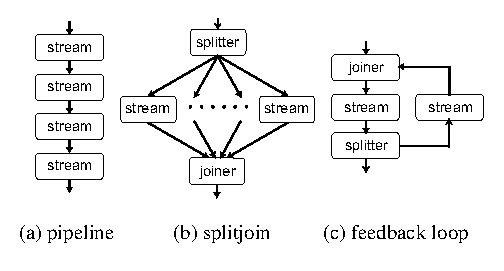
\includegraphics[scale=1, angle=0]{./constructs-eg.eps}
%}
% \vspace{-6pt}
% \nocaptionrule
 \caption{Hierarchical streams in StreamIt.}
 \label{fig:containers}
\end{center}
\end{figure}

\begin{figure}[t]
\begin{center}
\vspace{-12pt}
% \framebox{
 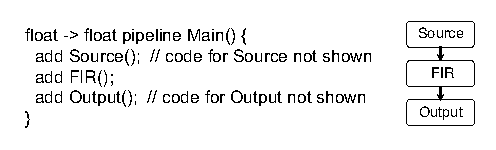
\includegraphics[scale=1, angle=0]{./pipeline-eg.eps}
%}
% \vspace{-6pt}
% \nocaptionrule
 \caption{Example pipeline with FIR filter.}
 \label{fig:pipeline}
%\vspace{-18pt}
\end{center}
\end{figure}

In StreamIt, the
application developer focuses on the hierarchical assembly of the
stream graph and its communication topology, rather than on the 
explicit management of the data buffers between filters.
StreamIt provides three hierarchical structures for composing filters
into larger stream graphs (see Figure~\ref{fig:containers}). The 
{\it pipeline} construct composes streams in sequence, with the output
of one connected to the input of the next.   An example of a pipeline
appears in Figure~\ref{fig:pipeline}.

The {\it splitjoin} construct distributes data to a set of parallel
streams, which are then joined together in a roundrobin fashion.  In
a splitjoin, the {\it splitter} performs the data scattering, and the
{\it joiner} performs the gathering. A splitter is a specialized
filter with a single input and  multiple output channels. On 
every execution step, it can distribute its output to any one of
its children in either a {\it duplicate} or a {\it roundrobin}
manner. For the former, incoming data are replicated to every
sibling connected to the splitter. For the latter, data are scattered
in a roundrobin manner, with each item sent to exactly one child
stream, in order.  The splitter type and the weights for distributing data to
child streams are declared as part of the syntax (e.g., \texttt{split
duplicate} or \texttt{split roundrobin($w_1,\ldots,w_n$)}). The
splitter counterpart is the joiner. It is a specialized filter with  
multiple input channels but only one output channel. The joiner
gathers data from its predecessors in a roundrobin manner (declared
as part of the syntax) to produce a single output stream.

StreamIt also provides a {\it feedback loop} construct for introducing
cycles in the graph.

%\section{Execution Model}
%\label{sec:execmodel}

%% A StreamIt program is represented by a hierarchical graph,
%% where the leaf nodes are filters, splitters, and joiners, and
%% the composite nodes are pipelines, splitjoins, and
%% feedback-loops. Edges in the graph represent data channels, which 
%% operate as FIFO queues.
\paragraph*{Execution Model}
As noted earlier, an actor (i.e., a filter, splitter, or joiner)
executes whenever there are enough data items on its input 
tape. In StreamIt, actors have  two epochs
of execution: one for initialization, and one for the {\it steady
state}. The initialization primes the input tapes to allow filters with
peeking to execute the very first instance of their work functions.
%%initialization in this setting is similar to the prologue stage in
%%software pipelining. 
A steady state is an execution that does not change the
buffering in the channels: the number of items on each channel
after the execution is the same as it was before the execution. 
Every valid stream graph has a steady state~\cite{LM87-i}, and within
a steady state, there are often many possibilities for interleaving
actor executions. 
%% The steady state schedule has the property that
%% the amount of data buffered between any two actors does not change
%% before and after the actor executions.
\begin{figure}[t]
\begin{center}
%%\vspace{-24pt}
%\vspace{24pt}
 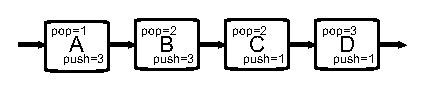
\includegraphics[scale=1, angle=0]{./pipe-with-rates.eps}
%\vspace{-6pt}
% \nocaptionrule
 \caption{Example pipeline.}
 \label{fig:pipe-with-rates}
\end{center}
%\vspace{-12pt}
\end{figure}
An example of a steady state for the pipeline in
Figure~\ref{fig:pipe-with-rates} requires filter \texttt{A} to fire
4 times, \texttt{B} 6 times, \texttt{C} 9 times, and
\texttt{D} 3 times. 
% Because in StreamIt the filters are
% independent (i.e., they do not share state), they can execute
% concurently. In a uniprocessor setting (which is what we use for our
% evaluation), we can only run one filter at time. Therefore, 
% The data generated by one actor are buffered (cached) until they are
% consumed.

\paragraph*{Compilation Process}
The StreamIt compiler derives the initialization and steady state
schedules~\cite{karczma-lctes03} and outputs a C program that includes
the initialization and work functions, as well as a driver to execute
each of the two schedules. Our compilation process allows the StreamIt
compiler to focus on high level optimizations, and relies on existing
compilers to perform machine-specific optimizations such as register
allocation, instruction scheduling, and 
code generation---this two-step approach affords us a
great deal of portability (e.g., code generated from the StreamIt
compiler is compiled and run on three different machines as reported
in Section~\ref{sec:evaluation}).

%% For example, referring to
%% Figure~\ref{fig:pipe-with-rates}, the compiler generates the following
%% sample code for running the steady state schedule:
%% %\begin{scriptsize}
%% \begin{verbatim}
%% run_steady_state() {
%%   for (i = 0; i < 4; i++) A_work();
%%   for (i = 0; i < 6; i++) B_work();
%%   for (i = 0; i < 9; i++) C_work();
%%   for (i = 0; i < 3; i++) D_work();
%% }
%% \end{verbatim}
%% %\end{scriptsize}
%% To execute the program, the steady state is wrapped with
%% another loop that invokes the steady state a designated number of
%% times. Preceding the state steady, a similar initialization schedule
%% is run to prime the data buffers.
%, and following the steady state, an
%epilogue is run to drain the buffers as necessary.

%% \begin{figure}[t]
%% \begin{center}
%% \vspace{-12pt}
%%  \psfig{figure=ssi.eps,width=3in}
%%  \vspace{-6pt}
%%  \caption{Instruction size (in bytes along the y-axis) per filter
%%  (x-axis) occurring in a steady state execution of FFT.}
%%  \label{fig:ssi-single}
%% \vspace{-18pt}
%% \end{center}
%% \end{figure}

\section{Cache Model for Streaming}
\label{sec:cache-model}

From a caching point of view, it is intuitively clear that once a
actor's instruction working set is fetched into the cache, we can
maximize instruction locality by running the actor as many times as
possible.  This of course assumes that the total code size for
all actors in the steady state exceeds the capacity of the
instruction cache.
%% In
%% Figure~\ref{fig:ssi-single} we show a representative breakdown of the
%% code size per actor in a steady state execution of a StreamIt
%% implementation of a Fast Fourier Transform (FFT).
For our benchmarks, the total code size for a steady state
ranges from 2~Kb to over 135~Kb (and commonly exceeds 16~Kb). Thus, while individual actors may have a
small instruction footprint, the total footprint of the actors in a
steady state exceeds a typical instruction cache size.
From these observations, it is evident that we must {\it scale} the
execution of actors in the steady state in order to improve temporal
locality. In other words, rather than running a actor $n$ times per
steady state, we scale it to run $m \times n$ times.
%
%% (e.g., the loop bound for \verb+A_work+ is
%% changed to $\texttt{m} \times 4$ in the example shown earlier). 
We term $m$ the {\it scaling factor}.

The obvious question is: to what extent can we scale the execution of
actors in the steady state? The answer is non-trivial because
scaling, while beneficial to the instruction cache behavior, may
overburden the data cache as the buffers between actors may grow to
prohibitively large sizes that degrade the data cache
behavior. Specifically, if a buffer overflows the cache, then
producer-consumer locality is lost.

In this section we describe a simple and intuitive cache model to
estimate the instruction and data cache miss rates for a steady state
sequence of actor firings. The model serves as a foundation for
reasoning about the cache aware optimizations introduced in this
paper. We develop the model first for the instruction cache, and then
generalize it to account for the data cache.

\subsection{Instruction Cache}

A steady state execution is a sequence of actor firings
$S=(a_1,\ldots, a_n)$, and a
{\it program execution} corresponds to one or more repetitions of the
steady state. We use the notation $S[i]$ to refer to the
actor $a$ that is fired at logical time $i$, and $|S|$ to
denote the length of the sequence. 

Our cache model is simple in that it considers each actor in the
steady state sequence, and determines whether one or more misses are
bound to occur. The miss determination is based on the 
the {\it instruction reuse distance} ($\mt{IRD}$), which is equal to
the number of unique instructions that are referenced between two
executions of the actor under consideration (as they appear in the
schedule). The steady state is a 
compact representation of the whole program execution, and thus, we
simply account for the misses within a steady state, and generalize
the result to the whole program. Within a steady state, an actor is
charged a miss penalty if and only if the number of referenced
instructions since the last execution (of the same actor)
is greater than the instruction cache capacity.

Formally, let $\mt{phase}(S,i)$ for $1\le i\le|S|$ represent a
subsequence of $k$ elements of $S$:
\[ 
\mt{phase}(S,i) = ( S[i], S[i+1], \ldots, S[i+k-1] )
\]
where $k\in[1,|S|]$ is the smallest integer such that $S[i+k]=S[i]$.
In other words, a phase is a subsequence of $S$ that starts with the
specified actor ($S[i]$) and ends before the next occurrence of the same actor
(i.e., there are no intervening occurrences of $S[i]$ in the phase).
Note that because the steady state
execution is cyclic, the construction of the subsequence is allowed to
wrap around the steady state\footnote{In other words, the subsequence
is formed from a new sequence $S'=S|S$ where $|$ represents
concatenation.}. For example, the steady state $S_1=(\texttt{AABB})$
has 
$\mt{phase}(S_1,1)=(\texttt{A})$,
$\mt{phase}(S_1,2)=(\texttt{ABB})$,
$\mt{phase}(S_1,3)=(\texttt{B})$, and
$\mt{phase}(S_1,4)=(\texttt{BAA})$,


Let $I(a)$ denote the code size of the work function for actor $a$.
Then the instruction reuse distance is
\[
%\mt{IRD}(S,i)=\sum_{j \in \mt{phase}(S,i)} I(S[j])
\mt{IRD}(S,i)=\sum_{a} I(a)
\]
where the sum is over all distinct actors $a$ occurring in
$\mt{phase}(S,i)$. We can then determine if a specific actor will
result in an instruction cache miss (on its next firing) by evaluating
the following step function:
\begin{equation}
\label{eq:imiss}
  \mt{IMISS}(S,i) =
    \begin{cases}
      0& \text{if $\mt{IRD}(S,i) \leq C_I$; hit: no cache refill,}\\
      1& \text{otherwise; miss: (some) cache refill.}
    \end{cases}
\end{equation}
In the equation, $C_I$ represents the instruction cache size. 

Using 
%the instruction miss ($\mt{IMISS}$) metric in
Equation~\ref{eq:imiss}, we can estimate the instruction miss
rate ($\mt{IMR}$) of a steady state as: 
\begin{equation}
\label{eq:imr}
  \mt{IMR}(S) = \frac{1}{|S|}\sum_{i=1}^{|S|} \mt{IMISS}(S,i).
\end{equation}

The cache model allows us to rank the quality of an
execution ordering: schedules that boost temporal locality
result in miss rates closer to zero, and schedules that do not
exploit temporal locality result in miss rates closer to one.

For example, in the steady 
state $S_1=(\texttt{AABB})$, assume that the combined instruction working
sets exceed the instruction cache, i.e., $I(\texttt{A}) + I(\texttt{B}) > C_I$.
Then, we expect to suffer a miss at the start of every
steady state because the phase that precedes the execution of
\texttt{A} (at $S_1[1]$) is $\mt{phase}(S_1,2)$ with 
an instruction reuse distance greater than the cache size 
($\mt{IRD}(S_1,2) > C_I$). Similarly, there is a 
miss predicted for the first occurrence of actor \texttt{B} since
$\mt{phase}(S_1,4)=(\texttt{BAA})$ and 
$\mt{IRD}(S_1, 4)>C_I$. Thus, $\mt{IMR}(S_1)=2/4$ whereas for the
following variant $S_2=(\texttt{ABAB})$, $\mt{IMR}(S_2)=1$.
In the case of $S_2$, we know that since the combined
instruction working sets of the actors exceed the cache size, when
actor \texttt{B} is fired following \texttt{A}, it evicts part of
actor \texttt{A}'s instruction working set. Hence when we transition
back to fire actor \texttt{A}, we have to refetch certain
instructions, but in the process, we replace parts of actor
\texttt{B}'s working set. In terms of our model, $\mt{IRD}(S_2,i)>C_I$
for every actor in the sequence, i.e., $1\le i\le|S_2|$.

Note that the
amount of refill is proportional to the number of cache lines that are
replaced when swapping actors, and as such, we may wish to adjust
our cache miss step function ($\mt{IMISS}$). One simple variation is to allow for
some partial replacement without unduly penalizing the overall value
of the metric. Namely, we can allow the constant $C_I$ to be some
fraction greater than the actual cache size. Alternatively, we can use
a more complicated miss function with a more uniform probability
distribution.

\paragraph*{Temporal Locality} In our model, the concept of improving
temporal instruction locality translates to deriving a steady state where, in the
best case, every actor has only one phase that is longer than unit-length.
For example, a permutation of the actors in $S_2$ (where all
phases are of length two) that improves temporal locality
will result in $S_1$, which we have shown has a relatively lower miss rate.


\paragraph*{Execution Scaling}
Another approach to improving temporal locality is to scale the
execution of the actors in the steady state. Scaling increases the
number of consecutive firings of the same actor. In our model, a
scaled steady state has a greater number of unit-length phases (i.e., a
phase of length one and the shortest possible reuse distance).

We represent a scaled execution of the steady state as
$S^m=(a_1^m,\dots, a_n^m)$: the steady state $S$ is scaled by $m$, which
translates to $m-1$ additional firings of 
every actor. For example, scaling $S_1=(\texttt{AABB})$ by a factor of
two results in
%$S_1^2=(\texttt{\underline{A}A\underline{A}A\underline{B}B\underline{B}B})$
$S_1^2=(\texttt{AAAABBBB})$
and scaling $S_2=(\texttt{ABAB})$ by the same amount results in 
%$S_2^2=(\texttt{\underline{A}A\underline{B}B\underline{A}A\underline{B}B})$.
$S_2^2=(\texttt{AABBAABB})$;
%; the underlined actors constitute the unscaled steady state.

From Equation~\ref{eq:imiss}, we observe that unit-length phases do
not increase the instruction miss rate  as long as the size of the actor's 
instruction working set  is smaller than the cache
size; we assume this is always the case. Therefore, scaling has the
effect of preserving the pattern of 
miss occurrences while also lengthening the steady state. Mathematically,
we can substitute into Equation~\ref{eq:imr}:
\begin{eqnarray}
  \nonumber
  \mt{IMR}(S^m)  &=& \frac{1}{|S^m|}\sum_{i=1}^{|S^m|} \mt{IMISS}(S^m,i) \\
  \nonumber
                 &=& \frac{1}{m \times |S|}\sum_{i=1}^{|S^m|} \mt{IMISS}(S^m,i). \\
  \label{eq:imrM}
                 &=& \frac{1}{m \times |S|}\sum_{i=1}^{|S|} \mt{IMISS}(S,i).
\end{eqnarray}
The last step is possible because $\mt{IMISS}$ is zero for $m-1$ out
of $m$ executions of every scaled actor.  The result is that the miss
rate is inversely proportional to the scaling factor.
\begin{figure}[t]
\begin{center}
  \psfig{figure=fftc-mult2.eps, width=\columnwidth}
% \nocaptionrule
  \caption{Impact of execution scaling on performance.}
 \label{fig:scaling-data}
\end{center}
\end{figure}

In Figure~\ref{fig:scaling-data} we show a
representative curve relating the scaling factor to overall
performance. The data corresponds to a coarse-grained implementation of 
a Fast Fourier Transform (FFT) running on a Pentium~3 architecture. The
x-axis represents the scaling factors (with increasing values from
left to right). The y-axis represents the execution time and is an
indirect indicator of the miss rate (the two measures are positively
correlated). The execution time improves in accord with our model: 
the running time is shortened as the scaling factor grows larger. There
is however an eventual degradation, and as the sequel will show, it is 
attributed to the data cache performance.

\subsection{Data Cache}

The results in Figure~\ref{fig:scaling-data} show that scaling can
reduce the running time of a program, but ultimately, it degrades
performance. In this section, we provide a basic analytical model that
helps in reasoning about the relationship between scaling and the data
cache miss rate. 

We distinguish between two types of data working sets. The static data
working set of an actor represents state, e.g., \texttt{weights} in
the FIR example (Figure~\ref{fig:fir}).  The dynamic data
working set is the data generated by the work function and pushed onto
the output channel. Both of these working sets impact the data cache
behavior of an actor.

Intuitively, the presence of state suggests that it is
prudent to maximize that working set's temporal locality. In this
case, scaling positively improves the data cache performance. To see
that this is true, we can define a data miss rate ($\mt{DMR}$) based on
a derivation similar to that for the instruction miss rate, replacing
$C_I$ with $C_D$ in Equation~\ref{eq:imiss}, and $I(a)$ with
$\mt{State}(a)$ when calculating the reuse distance. Here, $C_D$
represents the data cache size, and
$\mt{State}(a)$ represents the total size of the static data in the
specified actor. 

Execution scaling however also increases the I/O requirements of a
scaled actor. Let $\mt{pop}$ and $\mt{push}$ denote the declared pop and push rates
of an actor, respectively.  The scaling of an
actor by a factor $m$ therefore increases the pop rate to $m\times \mt{pop}$
and the push rate to $m\times \mt{push}$. Combined, we represent the dynamic
data working set of an actor $a$ as $\mt{IO}(a, m) =
m\times(\mt{pop}+\mt{push})$. Therefore, we measure the data reuse distance ($\mt{DRD}$)
of an execution $S$ with scaling factor $m$ as follows:
\[
  \mt{DRD}(S^m,i)=\sum_{a} \mt{State}(a) + \mt{IO}(a,m)
\]
where the sum is over all distinct actors $a$ occurring in $\mt{phase}(S^m,i)$.  While
this simple measure double-counts data that are both produced and
consumed within a phase, such duplication could be roughly accounted
for by setting $\mt{IO}'(a,m) = \mt{IO}(a,m) / 2$.

We can determine if a
specific work function will result in a data cache miss (on its next
firing) by evaluating the following step function:
\begin{equation}
\label{eq:dmiss}
  \mt{DMISS}(S^m,i) =
    \begin{cases}
      0& \text{if $\mt{DRD}(S^m,i) \leq C_D$; hit: no cache refill,}\\
      1& \text{otherwise; miss: (some) cache refill.}
    \end{cases}
\end{equation}
Finally, to model the data miss rate ($\mt{DMR}$):
\begin{eqnarray}
  \label{eq:dmrM}
  \mt{DMR}(S^m) &=& \frac{1}{|S^m|}\sum_{i=1}^{|S^m|} \mt{DMISS}(S^m,i).
\end{eqnarray}

It is evident from Equation~\ref{eq:dmrM} that scaling can lead to
lower data miss rates, as the coefficient $1/|S^m| = 1/(m \times |S|)$
is inversely proportional to $m$.  However, as the scaling factor $m$
grows larger, more of the $\mt{DMISS}$ values transition from $0$ to
$1$ (they increase monotonically with the I/O rate, which is
proportional to $m$).  For sufficiently large $m$, $\mt{DMR}(S^m) =
1$.  Thus, scaling must be performed in moderation to avoid negatively
impacting the data locality.

Note that in order to generalize the data miss rate equation so that it properly
accounts for the dynamic working set, we must consider the amount of
data reuse within a phase. This is because any actor that fires within
$\mt{phase(S,i)}$ might consume some or all of the data
generated by $S[i]$. The current model is simplistic, and leads to
exaggerated I/O requirements for a phase. We also do not model the
effects of cache conflicts, and take an ``atomic'' view of cache
misses (i.e., either the entire working set hits or misses).

%These observations suggest that in order to maximize the locality of
%any static data in an actor, the compiler should not only favor short
%phases, but also, it should schedule actor executions so that
%producer-consumer pairs appear within the same phase. Our cache-aware
%optimizations, described in the next section, exploits these
%observations.


%% Also complicating matters is the amount of state a actor must retain
%% from one execution of its work function to the next. In the FIR
%% example shown earlier, the state is proportional to the size of
%% the coefficient array (i.e., \texttt{weights}). Thus any scaling of
%% actor firings is further constrainted by the state.


%% We do not account for the cold start
%% effects of an execution trace. This does not affect our model, and can
%% be easily remedied if necessary. To see why this is so, consider the
%% following two execution traces which represent the executions of work
%% functions for two actors \texttt{A} and \texttt{B}:
%% $T_1 = \texttt{A}_1\texttt{A}_2\texttt{B}_3\texttt{B}_4$
%% and 
%% $T_2 = \texttt{A}_1\texttt{B}_2\texttt{A}_3\texttt{B}_4$.
%% In both 
%% traces, the number of cold starts is the same (i.e., two in all).


%% Note that different execution orderings for
%% the same stream graph lead to traces of the same size and hence the
%% comparisons are fair. 

%% Our model predicts that scaling the multipicitly of the actors always
%% leads to lower miss rates. An actor is fired a greater number of times in 
%% the steady state before transitioning to the next actor in the
%% schedule. Specifically, scaling a steady state $S$ by a multiplicity
%% factor $m$ 
%% Hence for example, a program that would generate a trace
%% $T_2$
%% might be as follows:
%% {\small
%% \begin{verbatim}
%% run_steady_state() {
%%   for (i = 0; i < 1; i++) A_work();
%%   for (i = 0; i < 1; i++) B_work();
%% }
%% \end{verbatim}}
%% \noindent but a scaled program that increases temporal locality is as follows:
%% {\small
%% \begin{verbatim}
%% run_steady_state() {
%%   for (i = 0; i < m * 1; i++) A_work();
%%   for (i = 0; i < m * 1; i++) B_work();
%% }
%% \end{verbatim}}
%% \noindent where \texttt{m} (the multiplicity factor) is an integer greater than
%% one.
%% From our model, it is easy to see that scaling reduces the number
%% of misses for a given actor $f$ from $K$ to $\frac{K}{\texttt{m}}- 1$, where $K =
%% \sum \mt{IMS}(f)$ for all occurrences of $f$ in  the execution trace.

%% \subsection{Remarks}

%% Note  that we can  combine the  instruction and  data cache  miss rate
%% equations to yield one measure that estimates the temporal locality of
%% a streaming computation.

%% Also note that while we use  an execution trace to describe our model,
%% it  is possible  to  calculate  the instruction  and  data cache  miss
%% metrics at  compile time.  To do so,  we can leverage  the hierarchical
%% StreamIt   representation  that  dictates   the  ordering   of  actor
%% executions.


%% Intuitively, the dynamic data accounts for the size of the buffer
%% required for writing new values, as well as the size of the buffer
%% necessary for reading values. It also adjusts for any
%% producer-consumer locality since the output buffer of one actor is
%% also the input buffer of its neighbor in the stream graph. What this
%% measure tells us is that we can scale the execution of a actor as
%% long as its buffer requirements (for reading and writing) do not
%% exceed the cache, and furthermore, as long as the input-output rates
%% between producer consumer pairs are not grossly mismatched. Managing the buffer 
%% requirements is important and motivates a series of cache
%% optimizations discussed in the next section. In the case of rate
%% mismatch, the metric tells us that the effective cache size is
%% reduced, or in other words, the data that is left over after a
%% producer-consumer firing must be preserved until a future occurrence of
%% the same pair of actors. This translates to lower data locality and
%% degrades cache performance.

%% Mathematically, the dynamic data measure is defined as:
%% \begin{eqnarray}
%%   \nonumber
%%   Y(f_i) &=&\sum_{f_k} min(W(f_k), U(f_k) \times A(f_k)) + \\
%%   \nonumber
%% 	   &&\sum_{f_k} min(R(f_k), O(f_k) \times A(f_k)) - \\
%%   \nonumber
%%          &&\sum_{f_s} min(R(f_s), O(f_s) \times A(f_s))
%% \end{eqnarray}
%% with $W(f)$ equal to the output buffer size reserved for writing data, $R(f)$
%% equal to the input buffer size reserved for reading data, $U(f)$ equal to the
%% {\tt push} rate (in bytes) of the actor, $O(f)$ equal to the {\tt pop} rate (in
%% bytes) of the actor, and $A(f)$ equal to the number of occurrences of
%% actor $f$ in $phase(f_i)$. Also note that the $Y(f_i)$ is defined
%% over all distinct occurrences of $f_k$ in the phase, and $f_s$
%% represents the actor that consumes the data produced by $f_k$ (i.e.,
%% it is $f_k$'s successor in the stream graph, and $f_k$--$f_s$
%% constitute a producer-consumer pair; $f_s$ is unique unless $f_k$ is a splitter).

%% The first summand in the equation above quantifies the address space
%% accessed for writing data. It is  equal to the lesser of the buffer size
%% reserved for output, and the total number of items produced by
%% the actor (i.e., the push rate multiplied by the number of times the
%% work function fired in the phase); this avoids over estimating the
%% address space when an exceedingly large buffer is reserved but only a
%% portion of it is used for writing in a phase.

%% The second term in the equation quantifies the referenced address space 
%% for reading the input data. This term is also the lesser of two
%% values: the input buffer size, and the total number of bytes referenced for
%% reading data.

%% The third term avoids double counting since the output buffer of one
%% actor is also the input buffer of its successor in the stream
%% graph. The term quantifies the amount of data that is consumed by the
%% producer's successor (which therefore releases a portion of the
%% address space for use by other actors in the phase).

\section{Cache Optimizations}
\label{sec:cache-opt}

In this section we describe two cache aware optimizations that
are geared toward improving the cache behavior of streaming programs. First, we
describe {\it execution scaling} which 
scales a steady state to improve instruction locality, subject to the
data working set constraints of the actors in the stream graph.
Second, we describe {\it cache aware fusion} which performs a series
of granularity adjustments to the actors in the steady state. The
fusion serves to $(i)$ reduce
the overhead of switching between actors, $(ii)$ create coarser
grained actors for execution scaling, and $(iii)$ enable novel
buffer management techniques between fused actors (see Section~\ref{sec:buffer}).

\subsection{Execution Scaling}
We have already alluded to execution scaling in previous
sections. As the instruction cache model shows, increasing the number
of consecutive firings of the same actor leads to lower instruction
cache miss rates. However, scaling increases the data buffers that are
maintained between actors. Thus it is prudent that we account for the
data working set requirements as we scale a steady state.

Our approach is to scale the entire steady state by a single
scaling factor, with the constraint that only a small percentage
of the actors overflow the data cache. Our two-staged algorithm is
outlined in Figure~\ref{fig:scaling-algo}.

First, the algorithm calculates the largest possible scaling factor
for every actor that appears in the steady state. To do this, it calculates the
amount of data produced by each actor firing and divides the available
data cache size by this data production rate. In addition, the
algorithm can toggle the effective cache size to account for various
eviction policies.

Second, it chooses the largest
factor that allows a fraction $p$ of the steady state actors to be
scaled safely (i.e., the cache is adequate for their I/O
requirements).  For example, the algorithm might calculate
$m_\texttt{A} = 10$,
$m_\texttt{B} = 20$, 
$m_\texttt{C} = 30$, and 
$m_\texttt{D} = 40$, for four actors in some steady state. That is,
scaling actor \texttt{A} beyond 10 consecutive iterations will cause
its dynamic I/O requirements to exceed the data cache. Therefore, the
largest $m$ that allows $p=90\%$ of the actors to be
scaled without violating the cache constraints is 10.
Similarly, to allow for the safe scaling of $p=75\%$ of the actors, the
largest factor we can choose is 20.

In our implementation, we use a 90-10 heuristic. In other words, we
set $p=90\%$. We empirically determined this value via a series of
experiments using our benchmark suite; see~\cite{janis-thesis} for
detailed results.
%Specifically, we varied the
%scaling factor across a wide range of values,
%and measured the resulting performance

Note that our algorithm adjusts the effective cache size that is
reserved for an actor's 
dynamic working set (i.e., data accessed via {\tt pop} and {\tt
push}). This adjustment allows us to control the fraction of the cache
that is used for reading and writing data---and affords some
flexibility in targeting various cache organizations.  For example,
architectures with highly associative and multilevel caches may benefit
from scaling up the effective cache size (i.e., $\alpha > 1$), whereas
a direct mapped cache that is more prone to conflicts may benefit from
scaling down the cache (i.e., $\alpha < 1$). In our implementation, we
found $\alpha=2/3$ to work well. However, we note that the optimal
choice for the effective cache size is a complex function of the 
underlying cache organization and possibly the application as well; 
this is an interesting issue that warrants further investigation.

\begin{figure}[t]
\begin{center}
\framebox{\parbox{3.25in}{
\mbox{} ~~~~// {\it Returns a scaling factor for steady state $S$} \\
\mbox{} ~~~~// - $c$ is the data cache size\\
\mbox{} ~~~~// - $\alpha$ is the fraction of $c$ dedicated for I/O\\%$(0 < \alpha)$\\
\mbox{} ~~~~// - $p$ is the desired percentile of all actors to be\\
\mbox{} ~~~~// ~~satisfied by the chosen scaling factor $(0 < p \le 1$)\\
\mbox{} ~~~~{\bf calculateScalingFactor}($S$, $c$, $\alpha$, $p$) \{\\
\mbox{} ~~~~~~~{\bf create} array $M$ of size $|S|$\\
\mbox{} ~~~~~~~{\bf for} $i$ = 1 to $|S|$ \{ \\
\mbox{} ~~~~~~~~~~$a = S[i]$\\
\mbox{} ~~~~~~~~~~// calculate effective cache size\\
\mbox{} ~~~~~~~~~~$c' = \alpha \times (c - \mt{State}(a))$\\
%\mbox{} ~~~~~~~~~~// estimate I/O requirements\\
%\mbox{} ~~~~~~~~~~$d = \mt{IO}(X)$\\
\mbox{} ~~~~~~~~~~// calculate scaling factor for $a$ such \\
\mbox{} ~~~~~~~~~~// that I/O requirements are close to $c'$\\
\mbox{} ~~~~~~~~~~$M[i] = {\bf round}(c'~/~\mt{IO}(a, 1))$\\
\mbox{} ~~~~~~~\} \\
\mbox{} ~~~~~~~{\bf sort} $M$ into ascending numerical order\\
\mbox{} ~~~~~~~$i = \lfloor~(1-p) \times |S|~\rfloor$ \\
\mbox{} ~~~~~~~{\bf return} $M[i]$\\
\mbox{} ~~~~\}
}}
\end{center}
\nocaptionrule
\caption{Our heuristic for calculating the scaling factor.}
\label{fig:scaling-algo}
\end{figure}



\subsection{Cache Aware Fusion}
In StreamIt, the granularity of actors is determined by the
application developer, according to 
the most natural representation of an algorithm. When compiling to a
cache-based architecture, the presence of a  large number of actors
exacerbates the transition overhead between work functions.
It is the role of the compiler  to adjust the granularity of
the stream graph to mitigate the execution overhead.

In this section we describe an actor coarsening technique we refer to
as {\it cache aware fusion} (CAF). When two actors are fused, they
form a new actor whose work function is equivalent to its constituents.
For example, let an actor \texttt{A} fire $n$
times, and an actor \texttt{B} fire $2n$ times per steady state:
$S^n=(\texttt{A}^n\texttt{B}^n\texttt{B}^n)$. Fusing \texttt{A} and
\texttt{B} results in an actor \texttt{F} that is equivalent to one 
firing of \texttt{A} and two 
firings of \texttt{B}; \texttt{F} fires $n$ times per steady state
$(S^n=(\texttt{F}^n))$.  In other terms, the work
function for actor \texttt{F} inlines the work functions of
\texttt{A} and \texttt{B}.

When two actors are fused, their executions are scaled such that the output
rate of one actor matches the input rate of the next. In the example,
\texttt{A} and \texttt{B} represent a producer-consumer pair of
filters within a pipeline, with filter \texttt{A}  
pushing two items per firing, and \texttt{B} popping one item per
firing. The fusion implicitly scales the execution of \texttt{B} so
that it runs twice for every firing of \texttt{A}.

%Fusion is important because it leads to coarser grained actors with
%I/O rates that are more closely matched to their
%neighbors. Furthermore, the fused actors themselves become the target
%the execution scaling which results in better producer-consumer locality.

Fusion also reduces the overhead of switching between
work functions. In our infrastructure, the steady state is a loop that
invokes the work functions via method calls. Thus, every pair of fused
actors eliminates a method call (per invocation of the actors). The impact on
performance can be significant, but not only because method calls are
removed: the fusion of two actors also enables the compiler to
optimize across function boundaries. In particular, for actors that
exchange only a few data items, the compiler can allocate the data
streams to registers. 
%For example, in the example above, the values
%produced by \texttt{A} may be passed to \texttt{B} via registers, rather
%than through memory. 
The data channel between fused actors is
subject to special buffer management techniques as described in the
next section.

There are, however, downsides to fusion. First, as more and more
actors are fused, the instruction footprint can dramatically increase,
possibly leading to poor use of the instruction cache. Second, fusion
increases the data footprint when the fused actors maintain state
(e.g., coefficient arrays and lookup tables). Our fusion algorithm is
cache aware in that it is cognizant of the instruction and data sizes.

The CAF algorithm uses a greedy fusion heuristic to determine which
filters should be fused. It continuously fuses actors until the
addition of a new actor causes the fused actor to exceed {\it either}
the instruction cache capacity, or a fraction of the data cache
capacity.  For the former, we estimate the instruction code size using
a simple count of the number of operations in the intermediate
representation of the work function.  For the latter, we allow the
state of the new fused actor to occupy up to 50\% of the data cache
capacity.

The algorithm leverages the hierarchical nature of the stream graph,
starting at the leaf nodes and working upward.  For pipeline streams,
the algorithm identifies the connection in the pipeline with the
highest steady-state I/O rate, i.e., the pair of filters that
communicate the largest number of items per steady state.  These two filters
are fused, if doing so respects the instruction and data cache constraints.
To prevent fragmentation of the pipeline, each fused filter is further
fused with its upstream and downstream neighbors so long as the
constraints are met.  The algorithm then repeats this process with the
next highest-bandwidth connection in the pipeline, continuing until no
more filters can be fused.  For splitjoin streams, the CAF algorithm
fuses all parallel branches together if the combination satisfies the
instruction and data constraints.  Partial fusion of a splitjoin is
not helpful, as the child streams do not communicate directly with
each other; however, complete fusion can enable further fusion in
parent pipelines.

%% This differs from that in
%% \cite{streamit-asplos} in that the algorithm
%% only considers vertical fusion (i.e., within a pipeline): horizontal
%% fusion is not beneficial from caching perspective. \framebox{Expand on this} \framebox{Emphasize order:  fuse then scale.}
%Second, since the 
%graph partitioning is limited to
%horizontal cuts, our actor coarsening optimizations employs a greedy
%algorithm instead of a dynamic programing methodology; this reduces
%compilation time. 

%% \begin{figure*}[t]
%% \begin{verbatim}
%% Pipeline:

%% Calculate number of partitions required for each child.
%% If for any child this is >1 then remember those partitions.

%% For each sequence (i..j) of children where for each child 
%% number of partitions is 1.

%% Interval(i,j) = "
%%     Find maximum bandwidth connection between children. (k, k+1)
%%     Consider partition (k..k+1) 
%%     If partition (k..k+1) does not satisfy the requirement then
%%         Call Interval(i,k) and Interval(k+1,j) to find two sets of partitions.

%%     Else Start with (k, k+1) fused try fusing up or down
%%         until can not fuse up and down let this be (l, m)
%%         Remember (l..m) as a partition.
%%         Use Interval(i,l) and Interval(m,j) to find partitions."

%% SplitJoin:

%% Consider splitter/joiner and all branches in a single partition.
%% If this satisfies requirements then return a single partion
%% else remember partitions corresponding to each branch as final
%% partitions.
%% \end{verbatim}
%% \caption{Pseudocode of a greedy algorithm to find partitions}
%% \label{fig:greedy}
%% \end{figure*}


\section{Buffer Management}
\label{sec:buffer}

\begin{figure}[t]
%% \begin{minipage}{1.7in}
%% \centering
%% \psfig{figure=fusion-pipeline.eps,width=0.7in}

%% \caption{Stream graph for a synthetic buffer test.\protect\label{fig:code-graph}}
%% \end{minipage}
%% \hspace{0.3in}
\centering
{\small
\begin{verbatim}
          void->void pipeline BufferTest {
            add Source();                 
            add FIR();                    
          }                               
                                          
          void->float filter Source {     
            work push 1 {                 
              push( ... );             
            } 
          }                               
                                          
          float->void filter FIR {        
            int PEEK = 4;                 
            work pop 1 peek PEEK {        
              float result = 0;           
              for (int i=1; i<PEEK; i++) {
                result += i*peek(i);      
              }                           
              pop();                      
              print(result);              
            }                             
          }                               
\end{verbatim}}
\vspace{-6pt}
\caption{Original StreamIt code for the buffer test.\protect\label{fig:code-orig}}
\end{figure}

A salient characteristic of stream programs is the use of FIFO
channels to communicate between parallel components.  Such channels
make explicit the communication between actors, allowing execution to
proceed in parallel or out-of-order so long as items are produced
before they are consumed.  FIFO channels also provide a natural
abstraction for the programmer, as complex modules can be assembled
from a set of small, reusable components.  For these reasons, it is
important to optimize the performance of communication channels.  An
efficient implementation enables a high-level abstraction for
composing actors without sacrificing performance.

Buffer management in StreamIt is more involved than some other stream
languages, due to the {\tt peek} operation.  The {\tt peek} operation
allows an actor to access an item on its input channel without
removing the item from the channel (removal is done via the {\tt pop}
operation).  The {\tt peek} functionality is very important for
components such as FIR (Finite Impulse Response) actors that access
data over a sliding window.  Because a given data item is accessed by
multiple iterations of the actor, there must be a persistent buffer
that stores items across executions.  In the context of a
uniprocessor, efficient buffer management translates to efficient
maintenance and addressing of this buffer in memory.  On a parallel
system, buffers can also be implemented using network links.

In this section, we explore two basic strategies for buffer management
in stream programs.  The first strategy, termed {\it modulation},
implements a traditional circular buffer that is indexed by wraparound
head and tail pointers.  The second strategy, termed {\it copy-shift},
avoids modulo operations by shifting the buffer contents after each
execution.  We demonstrate that, while a naive implementation of
copy-shift can be $2\times$ to $3\times$ slower than modulation, optimizations that
utilize execution scaling can boost the performance of copy-shift to
be significantly faster than modulation (51\% speedup on StrongARM,
48\% speedup on Pentium~3, and 5\% speedup on Itanium~2).

\begin{figure}[t]
%% \begin{minipage}{1.7in}
%% \centering
%% \psfig{figure=fusion-pipeline.eps,width=0.7in}

%% \caption{Stream graph for a synthetic buffer test.\protect\label{fig:code-graph}}
%% \end{minipage}
%% \hspace{0.3in}
\centering
{\small
\begin{verbatim}
   void->void filter BufferTest {       
     int PEEK = 4;                      
     float[4] BUFFER;                   
     int push_index = 0;                
     int pop_index = 0;                 
                                        
     prework {                          
       for (int i=0; i<PEEK-1; i++) {   
         BUFFER[push_index++] = ... ;
       }                                
     }                                  
                                        
     work {                             
       // run Source                    
       BUFFER[push_index] = ... ;
       push_index = (push_index+1) & 3;              
                                        
       // run FIR                       
       float result = 0;                
       for (int i=1; i<PEEK; i++) {     
         result += i*BUFFER[(pop_index+i) & 3];    
       }                                
       pop_index = (pop_index+1) & 3;     
       print(result);                   
     }                                  
   }                                    
\end{verbatim}}
\vspace{-6pt}

\caption{Fused buffer test using modulation buffer management.\protect\label{fig:code-modulation}}
\end{figure}


Our study is done in the context of a synthetic benchmark, shown in
Figure~\ref{fig:code-orig}.  
%As depicted in Figure~\ref{fig:code-graph}, 
The benchmark is a pipeline consisting of a simple source and an FIR
actor.  On each iteration, the source pushes a single item.  The FIR
actor calculates a weighted sum over {\tt PEEK} items of the input,
then pops a single item from the channel.  In our experiments, we vary
the {\tt PEEK} value from 1 to 128 items.

\begin{figure*}[t]
\vspace{-3pt}
\nocaptionrule
\begin{minipage}{2.2in}
\hspace{-0.1in}\psfig{figure=arm-buf.eps,width=2.4in}
\caption{Performance of buffer management strategies on a StrongARM.\protect\label{fig:buf-arm}}
\end{minipage}
\hspace{0.1in}
\begin{minipage}{2.2in}
\hspace{-0.1in}\psfig{figure=p3-buf.eps,width=2.4in}
\caption{Performance of buffer management strategies on a Pentium~3.\protect\label{fig:buf-p3}}
\end{minipage}
\hspace{0.1in}
\begin{minipage}{2.2in}
\hspace{-0.1in}\psfig{figure=i2-buf.eps,width=2.4in}
\caption{Performance of buffer management strategies on an Itanium~2.\protect\label{fig:buf-i2}}
\end{minipage}
\vspace{18pt}
\hrule
\begin{minipage}[t]{2.25in}
%% copy-shift
{\FusionFig
\begin{verbatim}


void->void filter BufferTest {
  int PEEK = 4;
  float[3] BUFFER;

  prework {
    for (int i=0; i<PEEK-1; i++) {
      BUFFER[i] = ... ;
    }
  }

  work {
    float[4] TEMP_BUFFER;
    int push_index = 3;
    int pop_index = 0;

    // copy from BUFFER to TEMP_BUFFER
    for (int i=0; i<3; i++) {
      TEMP_BUFFER[i] = BUFFER[i];
    }

    // run Source
    TEMP_BUFFER[push_index++] = ... ;
    
    // run FIR
    float result = 0;
    for (int i=1; i<PEEK; i++) {
      result += i*TEMP_BUFFER[pop_index+i];
    }
    pop_index++;
    print(result);

    // copy from TEMP_BUFFER to BUFFER
    for (int i=0; i<3; i++) {
      BUFFER[i] = TEMP_BUFFER[i+1];
    }
  }
}
\end{verbatim}}

\caption{Copy-shift strategy.\protect\label{fig:copy-shift}}
\end{minipage}
~~\vrule~~
\begin{minipage}[t]{2in}
%% copy-shift + scalar-replacement
{\FusionFig
\begin{verbatim}


void->void filter BufferTest {
  int PEEK = 4;
  float[3] BUFFER;

  prework {
    for (int i=0; i<PEEK-1; i++) {
      BUFFER[i] = ... ; 
    }
  }

  work {
    float TEMP_BUFFER_0;
    float TEMP_BUFFER_1;
    float TEMP_BUFFER_2;
    float TEMP_BUFFER_3;

    // copy from BUFFER to TEMP_BUFFER
    TEMP_BUFFER_0 = BUFFER[0];
    TEMP_BUFFER_1 = BUFFER[1];
    TEMP_BUFFER_2 = BUFFER[2];

    // run Source
    TEMP_BUFFER_3 = ... ;
    
    // run FIR
    float result = 0;
    result += 1*TEMP_BUFFER_1;
    result += 2*TEMP_BUFFER_2;
    result += 3*TEMP_BUFFER_3;
    print(result);

    // copy from TEMP_BUFFER to BUFFER
    BUFFER[0] = TEMP_BUFFER_1;
    BUFFER[1] = TEMP_BUFFER_2;
    BUFFER[2] = TEMP_BUFFER_3;
  }
}
\end{verbatim}}

\caption{Copy-shift with scalar-replacement.\protect\label{fig:code-scalar-replace}}
\end{minipage}
~~\vrule~~
\begin{minipage}[t]{2.25in}
%% copy-shift + scaling
{\FusionFig
\begin{verbatim}


void->void filter BufferTest {
  int PEEK = 4;
  float[3] BUFFER;

  prework {
    for (int i=0; i<PEEK-1; i++) {
      BUFFER[i] = ... ;
    }
  }

  work {
    float[32] TEMP_BUFFER;
    int push_index = 3;
    int pop_index = 0;

    // copy from BUFFER to TEMP_BUFFER
    for (int i=0; i<3; i++) {
      TEMP_BUFFER[i] = BUFFER[i];
    }

    // run Source 16 times
    for (int k=0; k<16; k++) {
      TEMP_BUFFER[push_index++] = ... ;
    }
    
    // run FIR 16 times
    for (int k=0; k<16; k++) {
      float result = 0;
      for (int i=1; i<PEEK; i++) {
        result += i*TEMP_BUFFER[pop_index+i];
      }
      pop_index++;
      print(result);
    }
      
    // copy from TEMP_BUFFER to BUFFER
    for (int i=0; i<3; i++) {
      BUFFER[i] = TEMP_BUFFER[i+16];
    }
  }
}
\end{verbatim}}

\caption{Copy-shift with execution scaling.\protect\label{fig:code-scaling}}
\end{minipage}
\vspace{-6pt}
\end{figure*}


\subsection{Modulation}

Figure~\ref{fig:code-modulation} illustrates a fused version of the
benchmark using modulation for buffer management.  For simplicity, we
illustrate each buffer management strategy as a source-to-source
transformation in StreamIt.  Each fused actor contains a {\tt
prework} function in which the source actor executes several times to
prime the communication channel with initial items, as well as a {\tt
work} function that represents the steady-state execution.

The modulation scheme uses a traditional circular-buffer approach.
Three variables are introduced: a {\tt BUFFER} to hold all items
transfered between the actors, a {\tt push\_index} to indicate the
buffer location that will be written next, and a {\tt pop\_index} to
indicate the buffer location that will be read next (i.e., the
location corresponding to {\tt peek(0)}).  The communication
primitives are translated as follows: 

{\scriptsize
\begin{verbatim}
push(val); ==>  BUFFER[push_index] = val;
                push_index = (push_index + 1) % BUF_SIZE;

pop();     ==>  pop_index = (pop_index + 1) % BUF_SIZE;

peek(i)    ==>  BUFFER[(pop_index + i) % BUF_SIZE]
\end{verbatim}}
\noindent The StreamIt compiler converts the modulo operations to
bitwise-and operations by scaling the buffer to a power of two.  Note
that if there are no {\tt peek} operations, then the buffer will be
empty following each execution of the downstream actor.  In this
case, the indices can be reset to zero at the start of each execution
and the modulo operations can be eliminated.  However, in our example
the FIR actor performs peeking, so the modulo operations are
needed.

{\bf Experimental setup.}  Figures~\ref{fig:buf-arm},~\ref{fig:buf-p3}
and~\ref{fig:buf-i2} illustrate the performance of various buffer
management strategies on a 137~Mhz StrongARM~1110, a 600~Mhz Pentium~3
and a 1.3~Ghz Itanium~2, respectively.  The figures illustrate the
execution time per $10^7$ outputs for the synthetic benchmark
(Figure~\ref{fig:code-orig}) across a range of {\tt PEEK} values.  To
ensure a fair comparison with the scalar replacement optimization
(Section~\ref{sec:scalar-replacement}), all loops in the original
actor are fully unrolled.

{\bf Evaluation.}  The time required for the modulation strategy
increases linearly with the peek rate.  This is expected, as there is
a constant overhead per peek operation.  Relative to the other
strategies, modulation performs noticeably better on the Itanium~2.
We attribute this to the six integer units on the Itanium~2; since
there is not much additional work in this benchmark, it can likely
process the modulo operations in parallel with other operations using
software pipelining.

\subsection{Copy-Shift}

The copy-shift strategy, illustrated in Figure~\ref{fig:copy-shift},
shifts the live items to the front of the buffer at the beginning of
each execution.  Because each execution starts writing to and reading from
the buffer at the same location, there is no need for the indices to
wraparound and the modulo operations can be eliminated.  This benefit
is compounded by additional optimizations enabled by the copy-shift
approach, as described in the subsequent sections.

However, the cost of this strategy comes in the copying operations: at
the start of each execution, $(\mbox{\it peek} - \mbox{\it pop})$
items are copied from the persistent {\tt BUFFER} to the beginning of
a local {\tt TEMP\_BUFFER}.  Subsequent operations reference
{\tt TEMP\_BUFFER}, and the live items are copied back to the {\tt
BUFFER} upon completion.  While these two variables could also be
combined into a single buffer, keeping them separate results in a
smaller live data set when the actor is not executing.

The communication primitives are translated as follows:

{\scriptsize
\begin{verbatim}
push(val); ==>  TEMP_BUFFER[push_index] = val;
                push_index = push_index + 1;

pop();     ==>  pop_index = pop_index + 1;

peek(i)    ==>  TEMP_BUFFER[pop_index + i]
\end{verbatim}}
\noindent Compared to the modulation scheme, the copy-shift strategy
references the {\tt TEMP\_BUFFER} and does not perform modulo
operations.

{\bf Evaluation.}  As shown in
Figures~\ref{fig:buf-arm},~\ref{fig:buf-p3} and~\ref{fig:buf-i2},
the unoptimized copy-shift strategy is the slowest strategy that we
evaluate.  Though the cost per peek operation is smaller than the
modulation scheme, the copying overhead per iteration also grows with
the peek rate and cancels out any savings; overall, copy-shift
performs from $2\times$ to $3\times$ slower than modulation.  The following sections
describe optimizations that can justify taking the copy-shift
approach.

\subsection{Copy-Shift with Scalar Replacement}
\label{sec:scalar-replacement}

The first optimization enabled by the copy-shift scheme is dubbed {\it
scalar replacement}.  In contrast to the modulation scheme, the
copy-shift approach can result in array operations that access the
same location on every execution of the actor.  The idea behind
scalar replacement is to fully unroll the loops in the actor, thereby
resolving each array index to an integer literal.  Then, since each
location is fully resolved at compile time, an $n$-length array can be
replaced by a set of $n$ scalar variables: one for each item in the
buffer.  This transformation is illustrated in
Figure~\ref{fig:code-scalar-replace}.

Scalar replacement offers several performance benefits. Scalar
variables can be register allocated, and as local variables they are
subject to a range of dataflow optimizations (constant propagation,
copy propagation, dead code elimination, etc.).  Replacing array
operations with scalars also eliminates array index calculations.
Despite these benefits, scalar replacement is nearly impossible to do
in a general-purpose language such as C because array contents might
be aliased with other pointers.  StreamIt arrays represent values that
are independent in memory, thereby facilitating this optimization.

Note that scalar replacement can only be applied when array indices
can be resolved to compile-time constants.  In the presence of unpredictable
control flow within an actor, or if the loops are too large to fully unroll,
then scalar replacement does not apply.

{\bf Evaluation.}  Compared to an unoptimized copy-shift strategy,
Figures~\ref{fig:buf-arm},~Figures~\ref{fig:buf-p3}
and~\ref{fig:buf-i2} illustrate that scalar replacement offers
modest gains on our synthetic benchmark.  At the maximum peek rate of
128, the StrongARM and Pentium~3 offer speedups of 16\% and 26\%,
respectively; these speedups are roughly uniform across all peek rates.
On the Itanium~2, speedups range from 5\% to 58\% depending on the
peek rate.  We conjecture that scalar replacement is more critical for
small actors that perform only a few operations.  Due to the high
communication-to-computation ratio in such actors, there could be
large gains from register-allocating and copy-propagating the
temporary variables.

\subsection{Copy-Shift with Execution Scaling}

A final optimization of the copy-shift strategy uses execution scaling
to dramatically decrease the overhead associated with copying the
buffer contents on each iteration.  In any actor, the number of items
inspected on one execution and saved for the next
execution is $(\mbox{\it peek} - \mbox{\it pop})$.  This represents
the number of items copied by the copy-shift scheme.  However, this
cost can be amortized by scaling the number of executions of the
downstream actor in the fused code.  By enclosing the body of the
actor in a loop, the $\mbox{\it peek}$ and $\mbox{\it pop}$ rates can
be made arbitrarily large, while $(\mbox{\it peek} - \mbox{\it pop})$
remains constant.

Thus, execution scaling reduces the fraction of time spent copying to
an arbitrarily small level.  In our study, we scale the executions of
an actor until $(\mbox{\it peek} - \mbox{\it pop}) \leq
\frac{1}{4}~\mbox{\it pop}$.  In the synthetic benchmark, this implies
that each actor body executes 16 times before the buffer contents are
shifted.  The code resulting from this transformation is shown in
Figure~\ref{fig:code-scaling}.

Note that due to the large loops introduced by execution scaling, it
cannot be used in combination with scalar replacement.  If the loops
were unrolled to resolve the array indices, there could be a negative
impact on the instruction cache.

{\bf Evaluation.}  As shown in Figures~\ref{fig:buf-arm}
and~\ref{fig:buf-p3}, the copy-shift approach with execution scaling
performs significantly better than modulation on the StrongARM and
Pentium~3.  At the maximum peek rate of 128, the StrongARM exhibits a
51\% speedup while the Pentium~3 shows a 48\%.  These speedups make
sense, as each peek operation is cheaper due to the eliminated modulo
operations (implemented as bitwise-and in the modulation scheme),
while the overhead from copying is reduced to a fraction of the
original copy-shift approach.

The gains are less substantial on Itanium~2, where the speedup at
$\mbox{\it peek} = 128$ is only 5\% (Figure~\ref{fig:buf-i2}).  We
attribute this to the relatively high performance of the modulation
approach on Itanium~2; due to the six parallel integer units, the
bitwise-and operation may not increase the critical path.  This
balance might be different in programs with higher integer workloads
within the actors.  Still, copy-shift with execution scaling does no
worse than modulation (on any architecture), and execution scaling
always offers a large speedup over the original copy-shift approach.

\subsection{Summary}

We conclude that copy-shift with execution scaling is the best buffer
management strategy for actors that utilize peeking.  This is somewhat
surprising because the unoptimized copy-shift strategy has large
overheads that result in a slowdown relative to a circular buffer with
modulation.  However, by leveraging the flexibility of the parallel
stream graph to perform execution scaling, the overheads are
amortized.  Compared to a plain circular buffer strategy, there are
significant improvements on StrongARM (51\% speedup) and Pentium~3
(48\% speedup), and respectable performance (5\% speedup) on
Itanium~2.

%% \subsection{Reusing Intermediate Storage Variables}

%% Once loops have been unrolled, actors have been fused into a
%% partition and arrays have been replaced with scalar variables we can
%% find approximations of live ranges for the new variables and use this
%% information to reduce stack space required by the partition's work
%% function.

%% We replace the scalar variables that have been created as a result of
%% destroying arrays with a minimal number of variables, where minimal
%% number is the maximum number of overlapping live ranges at any point
%% in the work function of the fused partition.

%% The above optimization improves data access locality.


\section{Experimental Evaluation}
\label{sec:evaluation}

In this section we evaluate the merits of the proposed cache aware
optimizations and buffer management strategies.  We use three
different architectures: a 137~MHz StrongARM~1110, a 600~MHz Pentium~3
and a 1.3~GHz Itanium~2. The StrongARM results reflect performance for
an embedded target; it has a 16~Kb L1 instruction cache, an 8~Kb L1 data
cache, and no L2 cache.  The StrongARM also has a separate 512-byte
minicache (not targeted by our optimizations).  The Pentium~3 and
Itanium~2 reflect desktop performance; they have a 16~Kb L1 instruction
cache, 16~Kb L1 data cache, and 256~Kb shared L2 cache.

Our benchmark suite (see Table~\ref{tab:benchmarks}) consists of
11 StreamIt applications. They are compiled with the StreamIt
compiler which applies the optimizations described in this paper, as
well as aggressive loop unrolling (by a factor of 128 for all
benchmarks) to facilitate scalar replacement
(Section~\ref{sec:buffer}).  The StreamIt compiler outputs a
functionally equivalent C program that is compiled with \texttt{gcc}
(v3.4, -O3) for the StrongARM and for the Pentium~3 and with
\texttt{ecc} (v7.0, -O3) for the Itanium~2.  Each benchmark is then
run five times, and the median user time is recorded.

As the StrongARM does not have a floating point unit, we converted all
of our floating point applications (i.e., every application except for
{\tt bitonic}) to operate on integers rather than floats.  In
practice, a detailed precision analysis is needed in converting such
applications to fixed-point.  However, as the control flow within
these applications is very static, we are able to preserve the
computation pattern for the sake of benchmarking by simply replacing
every floating point type with an integer type.

\begin{table}[t]
\vspace{6pt}
\nocaptionrule
\center
\label{tab:benchmarks}
{\scriptsize
\begin{tabular}{|l|l|c|} \hline
\hspace{-2pt}{\bf Benchmark}&\hspace{-2pt}{\bf Description}& \hspace{-6pt} {\bf \# of Actors} \hspace{-6pt} \\ \hline \hline
\hspace{-2pt}\texttt{bitonic	} &\hspace{-2pt}bitonic sort of 64 integers	&	972 \\ \hline
\hspace{-2pt}\texttt{fir	      } &\hspace{-2pt} finite impulse response (128 taps)&	132 \\ \hline
\hspace{-2pt}\texttt{fft-fine	} &\hspace{-2pt}fine grained 64-way FFT	&	267 \\ \hline
\hspace{-2pt}\texttt{fft-coarse}\hspace{-2pt} &\hspace{-2pt}coarse grained 64-way FFT	&	26 \\ \hline
\hspace{-2pt}\texttt{3gpp	} &\hspace{-2pt}3GPP Radio Access Protocol	&	105 \\ \hline
\hspace{-2pt}\texttt{beamformer} & \hspace{-2pt}beamformer with 64 channels and 1 beam & 197 \\ \hline
\hspace{-2pt}\texttt{matmult	} & \hspace{-2pt}matrix multiplication	&	48 \\ \hline
\hspace{-2pt}\texttt{fmradio	} & \hspace{-2pt}FM Radio with 10-way equalizer	&	49 \\ \hline
\hspace{-2pt}\texttt{filterbank}\hspace{-2pt} & \hspace{-2pt}filterbank program (8 bands, 32 taps / filter)	&	53 \\ \hline
\hspace{-2pt}\texttt{filterbank2}\hspace{-3pt}& \hspace{-2pt}independent filterbank (3 bands, 100 taps / filter) &	37 \\ \hline
\hspace{-2pt}\texttt{ofdm	 }& \hspace{-2pt}Orthogonal Frequency Division Multiplexor~\cite{spectrumware}	&	16 \\ \hline
\end{tabular}
}
\caption{Evaluation benchmark suite.}
\vspace{6pt}
\end{table}

We also made an additional modification in compiling to the StrongARM:
our execution scaling heuristic scales actors until their output
fills 100\% of the data cache, rather than 2/3 of the data cache as
described in Section~\ref{sec:cache-opt}.  This modification accounts
for the 32-way set-associative L1 data cache in the StrongARM.  Due to
the high degree of associativity, there is a smaller chance that the
actor outputs will repeatedly evict the state variables of the
actor, thereby making it worthwhile to further fill the data cache.
This observation yields up to 25\% improvement on some
benchmarks.

\begin{figure}[t]
\nocaptionrule
\begin{minipage}{3.35in}
\centering
\psfig{figure=arm1.eps,width=3.4in}
\vspace{-14pt}
\caption{Summary of results on a StrongARM.\protect\label{fig:arm-perf}}
~ \\ \vspace{3pt}

\psfig{figure=p3-1.eps,width=3.4in}
\vspace{-14pt}
\caption{Summary of results on a Pentium~3\protect\label{fig:p3-perf}}
~ \\ \vspace{3pt}

\psfig{figure=i2-1.eps,width=3.4in}
\vspace{-14pt}
\caption{Summary of results on an Itanium~2\protect\label{fig:i2-perf}}
\end{minipage}
\end{figure}

\paragraph*{Overall Speedup} 
The overall speedups offered by our techniques are illustrated in
Figure~\ref{fig:arm-perf} (StrongARM), Figure~\ref{fig:p3-perf}
(Pentium~3), and \ref{fig:p3-perf} (Itanium~2).  These graphs have two
bars: one for ``full fusion'', in which all actors are fused into a
single function (with scalar replacement), and one labeled {\tt
CAF+scaling+buffer}, representing all of our optimizations (cache
aware fusion, execution scaling, and buffer optimizations) applied
together.  We include the comparison to full fusion because it
represents a simple approach for eliminating function call overhead
and optimizing across actor boundaries; while this fusion strategy
utilizes our scalar replacement optimization, it remains oblivious to
instruction and data locality.  Performance is normalized to
unoptimized StreamIt, in which no actors are fused (but there is
still unrolling by 128).  On the right of each graph, both arithmetic
and geometric means are shown for the benchmarks.  We usually speak in
terms of the arithmetic means as they are more intuitive (and also
yield more conservative speedups), though we refer to the geometric
mean for an unambiguous reference on close results.

On StrongARM (Figure~\ref{fig:arm-perf}), our cache optimizations
offer a 249\% average speedup over the baseline and a 162\% average
speedup over full fusion.  Scalar replacement is responsible for much
of the gains that both strategies offer over the baseline.  Cache
optimizations always perform better than the baseline, and they
perform better than full fusion in all cases except for \texttt{3gpp},
where they yield a 45\% slowdown.  This slowdown is due to
conservative code size estimation: the compiler predicts that the
fused version of \texttt{3gpp} will not fit into the instruction
cache, thereby preventing fusion.  However, due to optimizations by
{\tt gcc}, the final code size is smaller than expected and does fit
within the cache.  While such inaccuracies could be improved by adding
feedback between the output of {\tt gcc} and our code estimation, each
fusion possibility would need to be evaluated separately as the fusion
boundary affects the impact of low-level optimizations (and thus the
final code size).

The speedups offered by cache optimizations over a full fusion
strategy are more modest for the desktop processors: 34\% average
speedup on Pentium~3 (Figure~\ref{fig:p3-perf}) and essentially zero
speedup (6\% by the arithmetic mean, -8\% by the geometric mean) on
Itanium~2 (Figure~\ref{fig:i2-perf}).  Out of the 11 benchmarks, cache
optimizations perform as well or better than full fusion for 7
benchmarks on the Pentium~3 and 5 benchmarks on the Itanium~2.
Performance on any architecture is a tradeoff between two factors: 1)
the benefit of data and instruction locality, and 2) the benefit of
fusion, which reduces memory accesses due to improved register
allocation across actor boundaries.  Compared to the StrongARM, the
Pentium~3 and Itanium~2 offer an L2 cache (as well as a larger L1 data
cache), thereby lessening the impact of locality-enhancing cache
optimizations.  However, the fusion benefit remains a significant
factor; for example, using Intel VTune on the Pentium~3, we measured
that full fusion offers a 50\% reduction in memory accesses over the
cache-optimized version.  This effect may be pronounced on the Itanium~2
due to the larger number of registers on that architecture (128
general, 128 floating point).  While fusion benefits are also present
on the StrongARM, cache optimizations are more important on that processor
due to the large penalty for cache misses.

The cache aware fusion algorithm can be adjusted to account for the
caching hierarchy on desktop machines.  Specifically, if cache aware
fusion is modified to allow fused actors to consume up to one half of
the L2 cache (rather than L1 cache), then the performance of the cache
optimizations is closer or equal to full fusion, for cases it was
previously trailing on the Pentium~3 or the Itanium~2 (data not shown).  The
only benchmark that is negatively impacted by this change is {\tt
ofdm}, where two large actors are fused despite a very low
communication to computation ratio, thereby lessening the impact of
eliminated memory accesses while nonetheless worsening the instruction
locality.

\begin{figure}[t]
\nocaptionrule
\begin{minipage}{3.35in}
\centering
\psfig{figure=arm2.eps,width=3.4in}
\vspace{-14pt}
\caption{Impact of each optimization on a StrongARM.\protect\label{fig:arm-perf2}}
~ \\ \vspace{3pt}

\psfig{figure=p3-2.eps,width=3.4in}
\vspace{-14pt}
\caption{Impact of each optimization on a Pentium~3.\protect\label{fig:p3-perf2}}
~ \\ \vspace{3pt}

\psfig{figure=i2-2.eps,width=3.4in}
\vspace{-14pt}
\caption{Impact of each optimization on an Itanium~2.\protect\label{fig:i2-perf2}}
\end{minipage}
\end{figure}

\paragraph*{Impact of Each Optimization}
To better understand the overall speedups, we assess the individual
performance impact of execution scaling, cache aware fusion, and
buffer management optimizations.  These results are illustrated in
Figures~\ref{fig:arm-perf2}, \ref{fig:p3-perf2} and~\ref{fig:i2-perf2}
for the StrongARM, Pentium~3, and Itanium~2, respectively.  There are
four bars per benchmark; as in the previous analysis, all performance
is normalized to unoptimized StreamIt (with 128-way unrolling).  The
first bar, labeled {\tt scaling}, applies only execution scaling.  The
second bar, labeled {\tt CAF}, applies only cache aware fusion,
including scalar replacement across the fused actors.  The third bar,
labeled {\tt CAF+scaling}, first applies cache aware fusion with
scalar replacement and then applies execution-scaling to the
granularity-adjusted actors.  The fourth bar, labeled {\tt
CAF+scaling+buffer}, additionally applies buffer management
optimizations (detailed later); this bar is equivalent to the ``best''
cache-optimized performance illustrated in Figures~\ref{fig:arm-perf},
\ref{fig:p3-perf}, and \ref{fig:i2-perf}.

Execution scaling improves performance over unoptimized StreamIt, with
average speedups of 145\% for StrongARM, 58\% for Pentium~3, and 57\%
for Itanium~2.  The 90-10 heuristic works quite well
(see~\cite{janis-thesis} for full details) and there is only one
instance where scaling results in a performance degradation. The
granularity-adjusted \texttt{3gpp} on StrongARM has a 17\% slowdown
due to scaling (compare {\tt CAF} to {\tt CAF+scaling} in
Figure~\ref{fig:arm-perf}).  This is possibly due to items in flight
between the granularity-adjusted actors overwriting the state of an
executing actor in the data cache.  Since StrongARM has no L2 cache
then such eviction can be quite expensive.

Independently, cache aware fusion also improves performance by 84\% on
StrongARM, 101\% on Pentium~3 and a 103\% on the Itanium~2.
cache aware fusion degrades performance only for
\texttt{filter}-\texttt{bank2} (by 6\% on StrongARM). When we combine
cache aware fusion with execution scaling, the performance
consistently improves.  The speedup of \texttt{CAF+scaling} over
baseline is 241\% on StrongARM, 146\% on Pentium~3 and 144\% on
Itanium~2.

However, after coarsening the actors with cache aware fusion, scaling
results in less additional speedup than it did relative to the
baseline.  The speedup of \texttt{CAF+scaling} over \texttt{CAF} is
86\% for StrongARM, 22\% for Pentium~3 and only 20\% for Itanium~2.
This is because some actors are implicitly scaled by fusion to match
input/output rates of successive actors within a fused block.

Note that the \texttt{ofmd} benchmark does not benefit from fusion or
scaling. This is because \texttt{ofmd} has few actors, some of which
consume and produce a total of 16-66~Kb data; consequently, execution
scaling does not apply.  Also there is limited opportunity to fuse
actors within \texttt{ofmd}, as there are actors that have an
instruction size of 9~Kb and fusing them with other actors would
exceed the instruction cache.

The last bar, {\tt CAF+scaling+buffer}, illustrates the benefit of
buffer management optimizations for filters that peek.  As detailed in
Section~\ref{sec:buffer}, such filters demand specialized buffer
management, as they reuse items on the input tape across successive
iterations.  In our benchmark suite, peeking occurs only in the last
four applications (i.e., \texttt{fmradio}, \texttt{filterbank},
\texttt{filterbank2} and \texttt{ofdm}).  Thus, the {\tt CAF+scaling}
bar is equivalent to {\tt CAF+scaling+buffer} for all benchmarks from
{\tt bitonic} through {\tt matmult}.

The buffer optimization applied in Figures~\ref{fig:arm-perf},
\ref{fig:p3-perf}, and \ref{fig:i2-perf} is termed {\tt cutpeek}.  In
this optimization, the cache aware fusion algorithm is modified so
that two adjacent filters are never fused if the downstream filter
performs any peeking (i.e., it has $\mbox{\it peek} > \mbox{\it
pop}$).  Following execution scaling, the live items are copied to the
start of the buffer once per scaled execution (using the copy-shift
strategy, Section~\ref{sec:buffer}), thereby reducing the overhead
of copying live items.  Optimized buffer management offers the largest
gains for {\tt filterbank2}: 45\% on StrongARM, 38\% on Pentium~3, and
36\% on Itanium~2.  This is due to a large peek rate (100 items) in
addition a large scaling factor of 300 that amortizes the cost of
copying items.

While we found that {\tt cutpeek} is, on average, the best buffer
management strategy across the three platforms, we also evaluated
several others.  For {\tt fmradio}, up to a 5\% improvement is offered
by a strategy called {\tt peekscale}, in which (prior to other
optimizations) filters with $\mbox{\it peek}>\mbox{\it pop}$ are
scaled to perform several executions at once.  As scaling is
performed, the {\it pop} and {\it peek} rates increase but $\mbox{{\it
peek}} - \mbox{\it pop}$ remains constant; scaling continues until the
{\it pop} rate is at least $4*(\mbox{{\it peek}} - \mbox{{\it pop}})$.
Like {\tt cutpeek}, this serves to amortize the overhead of
copy-shift, but it can also hamper the execution scaling optimization.
Because certain other actors in the graph must fire more frequently to
compensate for the scaled peeking filter, there is less room for
global execution scaling.  The only other case where {\tt peekscale}
is the best strategy is for {\tt ofdm} on StrongARM, where there is a
7\% improvement over {\tt cutpeek}.  Finally, on the {\tt filterbank}
benchmark, highest performance results from unoptimized copy-shift
buffer management.  We also evaluated buffer management using
modulation for indexing, but this did not yield the best performance
for any benchmark or platform.

\section{Related Work}
\label{sec:related-work}

There is a large body of literature on scheduling synchronous dataflow
(SDF) graphs to optimize various
metrics~\cite{bhattacharyya99synthesis,leesdf}.  The work most closely
related to ours is a recent study by Kohli~\cite{kohli04} on
cache aware scheduling of SDF graphs, implemented as part of the
Ptolemy framework for simulating heterogeneous embedded
systems~\cite{ptolemy03overview}.  Kohli develops a Cache Aware
Scheduling (CAS) heuristic for an embedded target with a
software-managed scratchpad instruction cache.  His algorithm greedily
decides how many times to execute a given actor based on estimates of
the data cache and instruction cache penalties associated with
switching to the next actor.  In contrast, our algorithm considers the
buffering requirements of all filters in a given container and
increases the multiplicity so long as 90\% of buffers are contained
within the data cache.  Kohli does not consider buffer management
strategies, and the evaluation is limited to one 6-filter pipeline and
an assortment of random SDF graphs.  An empirical comparison of our
heuristics on a common architectural target would be an interesting
direction for future work.

It is recognized that there is a tradeoff between code size and buffer
size when determining an SDF schedule.  Most techniques to date have
focused on ``single appearance schedules'' in which each filter
appears at only one position in the loop nest denoting the schedule.
Such schedules guarantee minimal code size and facilitate the inlining
of filters.  There are a number of approaches to minimizing the buffer
requirements for single-appearance schedules (see
\cite{bhattacharyya99synthesis} for a review).  While it has been
shown that obtaining the minimal memory requirements for general
graphs is NP-complete~\cite{Bhatta97}, there are two complimentary
heuristics, APGAN (Pairwise Grouping of Adjacent Nodes) and RPMC
(Recursive Partitioning by Minimum Cuts), that have been shown to be
effective when applied together~\cite{Bhatta97}.  Buffer
merging\cite{murt1999x3,murt2000x2} represents another technique for
decreasing buffer sizes, which could be integrated with our approach
in the future.

Govindarajan et al. develop a linear programming framework for
determining the ``rate-optimal schedule'' with the minimal memory
requirement~\cite{GGD94}.  A rate-optimal schedule is one that takes
advantage of parallel resources to execute the graph with the maximal
throughput.  However, the technique is specific to rate-optimal
schedules and can result in a code size explosion, as the same node
is potentially executed in many different contexts.

The work described above is related to ours in that minimizing buffer
requirements can also improve caching behavior.  However, our goal is
different in that we aim to improve spatial and temporal locality
instead of simply decreasing the size of the live data set.  In fact,
our scaling transformation actually {\it increases} the size of the
data buffers, leading to higher performance across our benchmark
suite.  Our transformations also take into account the size of the
instruction and data caches to select an appropriate scaling and
partitioning for the stream graph.

Proebsting and Watterson \cite{pro96} give a fusion algorithm that
interleaves the control flow graphs of adjacent filters.  However,
their algorithm only supports synchronous {\tt get} and {\tt put}
operations; StreamIt's {\tt peek} operation necessitates buffer
management between filters.

There are a large number of stream programming languages; see
\cite{survey97} for a review.  The Brook language~\cite{Buck04}
extends C to include data-parallel kernels and multi-dimensional
streams that can be manipulated via predefined operators.  Synchronous
languages such as Esterel~\cite{esterel92} and LUSTRE~\cite{lustre}
also target the embedded domain, but they are more control-oriented
than StreamIt and are less amenable to compile-time optimizations.
Benveniste et al.~\cite{benveniste93dataflow} also provides an
overview of dataflow synchronous languages.  Sisal (Stream and
Iteration in a Single Assignment Language) is a high-performance,
implicitly parallel functional language~\cite{sisal}.  We are not
aware of any cache aware optimizations in these stream languages.

%(cache models?)
%[rodric:] there isn't a good survey/single source (that i know of) that covers
%cache miss equations and the like; are we ok with only giving the
%most important reference? i think so
There is a large body of work covering cache miss equations, and an
equally large body of work concerned with analytical models for
reasoning about data reuse distances and cache behavior. 
The model introduced in this paper is loosely based on the notion of
stack reuse distances~\cite{mattson70}.  Our model is especially tailored 
to streaming computations, and unique
in leveraging the concept of a steady state execution.

\section{Conclusions}
\label{sec:conclusion}

In this paper, we present a simple yet highly effective methodology
for running streaming programs on common cache-based architectures.
The work shows that we can exploit the abundant parallelism in
streaming codes to improve the behavior of the cache hierarchy and
deliver significant performance improvements on existing machines. We
evaluate our methodology on three architectures: the embedded
StrongARM processor, the superscalar Pentium~3, and the VLIW Itanium~2.

Our optimizations are simple but yield surprisingly big savings in
performance. First, we introduce {\it execution scaling}, which 
increases the execution frequency of every actor in the stream
graph. Intuitively, scaling improves instruction  locality because
it increases the amount of reuse from the instruction
cache. Concomitantly, it leads to performance gains of 145\% on the
StrongARM, 58\% on the Pentium~3, and 57\% on the Itanium~2.
It is worthy to note that execution scaling is a departure from
past optimization strategies for streaming programs, which try to
minimize buffer requirements. Our scaling transformation actually {\it
increases} the size of the data buffers between actors.

We also showed that scaling presents a tradeoff between 
instruction locality and data locality. Using a simple cache
model, we show how scaling impacts the instruction and data
caches. The model serves to motivate a heuristic for calculating the
scaling factor. The heuristic, which accounts for the size of the
instruction and data caches, works quite well in practice.

This paper also introduces {\it cache aware fusion}. The fusion
optimization helps to reduce the data requirements of a program, and
can reduce the total number of memory requests by as much as 50\%. The
fusion of actors in the stream graph is carried out judiciously, and
our algorithms are sensitive to the instruction and data working sets
of the coarsened execution units, as well as their impact on the cache
hierarchy. Cache aware fusion leads to performance gains of 84\% on
the StrongARM, 101\% on the Pentium~3, and 103\% on the Itanium~2.

Cache aware fusion also enables a set of novel buffer management
strategies for handling the streams of data between actors. Due to the
static nature of stream programs, we can often apply {\it scalar
  replacement} to remove array references, and thus communication
between fused actors is done through registers, rather than through
memory.  To allow scalar replacement to apply to sliding window 
computations, we introduce a {\it copy-shift} buffer management policy
that out-performs a traditional rotating buffer.

In summary, the application of execution scaling, cache aware fusion, and our
new buffer management strategies, can improve performance of
StreamIt programs by 249\% on the StrongARM, 154\% on the Pentium~3,
and 152\% on the Itanium~2.


\section{Acknowledgments}
We thank Michael Gordon and Jasper Lin for their helpful comments as 
well as their contributions to the StreamIt infrastructure.
The StreamIt project is
supported by DARPA grants PCA-F29601-03-2-0065 and
HPCA/PERCS-W0133890; NSF awards CNS-0305453 and EIA-0071841; and the
MIT Oxygen Alliance.

\begin{thebibliography}{10}

\bibitem{benveniste93dataflow}
A.~Benveniste, P.~Caspi, P.~L. Guernic, and N.~Halbwachs.
\newblock {Data-Flow Synchronous Languages}.
\newblock In {\em {REX} School/Symposium}, pages 1--45, 1993.

\bibitem{esterel92}
G.~Berry and G.~Gonthier.
\newblock {The Esterel Synchronous Programming Language: Design, Semantics,
  Implementation}.
\newblock {\em Science of Computer Prog.}, 19(2), 1992.

\bibitem{Bhatta97}
C.~S. Bhattacharyya, P.~K. Murthy, and E.~A. Lee.
\newblock {APGAN and RPMC: Complementary Heuristics for Translating DSP Block
  Diagrams into Efficient Software Implementations}.
\newblock {\em Journal of Design Automation for Embedded Systems.}, pages
  33--60, January 1997.

\bibitem{bhattacharyya99synthesis}
S.~Bhattacharyya, P.~Murthy, and E.~Lee.
\newblock Synthesis of embedded software from synchronous dataflow
  specifications.
\newblock {\em Journal of VLSI Signal Processing Systems}, 21(2), June 1999.

\bibitem{leesdf}
S.~S. Bhattacharyya, P.~K. Murthy, and E.~A. Lee.
\newblock {\em {Software Synthesis from Dataflow Graphs}}.
\newblock Kluwer Academic Publishers, 1996.

\bibitem{Buck04}
I.~Buck, T.~Foley, D.~Horn, J.~Sugerman, K.~Fatahalian, M.~Houston, and
  P.~Hanrahan.
\newblock {Brook for GPUs: Stream Computing on Graphics Hardware}.
\newblock In {\em SIGGRAPH}, 2004.

\bibitem{GGD94}
R.~Govindarajan, G.~Gao, and P.~Desai.
\newblock Minimizing memory requirements in rate-optimal schedules.
\newblock In {\em Proceedings of the 1994 Int. conference on Application
  Specific Array Processors}, pages 75--86, August 1994.

\bibitem{lustre}
N.~Halbwachs, P.~Caspi, P.~Raymond, and D.~Pilaud.
\newblock {The synchronous data-flow programming language LUSTRE}.
\newblock {\em Proc. of the IEEE}, 79(9), 1991.

\bibitem{sisal}
{J. Gaudiot and W. Bohm and T. DeBoni and J. Feo and P. Mille}.
\newblock {The Sisal Model of Functional Programming and its Implementation}.
\newblock In {\em Proc. of the Second Aizu International Symposium on Parallel
  Algorithms/Architectures Synthesis}, 1997.

\bibitem{karczma-lctes03}
M.~Karczmarek, W.~Thies, and S.~Amarasinghe.
\newblock Phased scheduling of stream programs.
\newblock In {\em LCTES}, 2003.

\bibitem{kohli04}
S.~Kohli.
\newblock Cache aware scheduling of synchronous dataflow programs.
\newblock Master's Report Technical Memorandum UCB/URL M04/03, UC Berkeley,
  2004.

\bibitem{ptolemy03overview}
E.~A. Lee.
\newblock {Overview of the Ptolemy Project}.
\newblock Technical report, Tech Memo UCB/ERL M03/25, UC Berkeley, 2003.

\bibitem{LM87-i}
E.~A. Lee and D.~G. Messerschmitt.
\newblock Static scheduling of synchronous data flow programs for digital
  signal processing.
\newblock {\em IEEE Transactions on Computers}, January 1987.

\bibitem{mattson70}
R.~L. Mattson, J.~Gecsei, D.~R. Slutz, and I.~L. Traiger.
\newblock Evaluation techniques for storage hierarchies.
\newblock {\em IBM Systems Journal}, 1970.

\bibitem{murt1999x3}
P.~K. Murthy and S.~S. Bhattacharyya.
\newblock {A Buffer Merging Technique for Reducing Memory Requirements of
  Synchronous Dataflow Specifications}.
\newblock In {\em International Symposium on System Synthesis}, 1999.

\bibitem{murt2000x2}
P.~K. Murthy and S.~S. Bhattacharyya.
\newblock {Buffer Merging --- A Powerful Technique for Reducing Memory
  Requirements of Synchronous Dataflow Specifications}.
\newblock Technical report, Inst. for Adv. Computer Studies, UMD College Park,
  2000.

\bibitem{pro96}
T.~A. Proebsting and S.~A. Watterson.
\newblock {Filter Fusion}.
\newblock In {\em POPL}, 1996.

\bibitem{janis-thesis}
J.~Sermulins.
\newblock In preparation.
\newblock Master's thesis, MIT CSAIL, 2005.

\bibitem{survey97}
R.~Stephens.
\newblock {A Survey of Stream Processing}.
\newblock {\em Acta Informatica}, 34(7), 1997.

\bibitem{spectrumware}
D.~Tennenhouse and V.~Bose.
\newblock {The SpectrumWare Approach to Wireless Signal Processing}.
\newblock Wireless Networks, 1999.

\bibitem{streamitcc}
W.~Thies, M.~Karczmarek, and S.~Amarasinghe.
\newblock {StreamIt: A Language for Streaming Applications}.
\newblock In {\em {Proc. of the Int. Conf. on Compiler Construction (CC)}},
  {2002}.

\end{thebibliography}

%% \clearpage

%% \begin{figure*}[t]
%%   \begin{center}
%%     {\Large
%%       {\bf APPENDIX: OPTIONAL MATERIAL}
%%     }
%%   \end{center}

%%   \hspace{-10pt}\psfig{figure=beam-mult.eps,width=2.5in}\hspace{-20pt}
%%   \psfig{figure=bisort-mult.eps,width=2.5in}\hspace{-20pt}
%%   \psfig{figure=fbank-mult.eps, width=2.5in}\hspace{-20pt}
%%   \vspace{-24pt}

%%   \hspace{-10pt}\psfig{figure=fftc-mult.eps,  width=2.5in}\hspace{-20pt}
%%   \psfig{figure=fftf-mult.eps,  width=2.5in}\hspace{-20pt}
%%   \psfig{figure=3gpp-mult.eps,    width=2.5in}\hspace{-20pt}
%%   \vspace{-24pt}

%%   \hspace{-10pt}\psfig{figure=fir-mult.eps,    width=2.5in}\hspace{-20pt}
%%   \psfig{figure=matmult-mult.eps,    width=2.5in}\hspace{-20pt}
%%   \psfig{figure=fm-mult.eps,    width=2.5in}\hspace{-20pt}
%%   \caption{Execution time in seconds as a function of multiplicity scaling on a
%%   Pentium~3.}
%%   \label{fig:9010}
%% \end{figure*}

\end{document}
